\section{Proof}
\subsection{Proof of Property~\ref{p1}}
\label{subsection:proof1}
\begin{proof}
	Without loss of generality, we assume that the weights that voter $a_i$
	values all DApps are $b_{i1}, b_{i2}, \ldots, b_{in}$ respectively, which are
	fixed. We assume that voter $a_i$'s contributory values to all DApps are
	$\nr_{i1},\ldots,\nr_{in}$ respectively, which are adjustable by voter $a_i$.

	The optimization objective of voter $i$ is the weighted sum of ranking scores that he offers, defined by
	$$w_i = \sum_{j=1}^n b_{ij}\sqrt{\nr_{ij}}$$
	According to Cauthy's inequality it holds that
	$$w_i = \sum_{j=1}^n b_{ij}\sqrt{\nr_{ij}} \leq (\sum_{j=1}^n b_{ij}^2)(\sum_{j=1}^n \nr_{ij}) \leq (\sum_{j=1}^n b_{ij}^2)\nr_i$$
	The most right side of the formula	above is a fixed value. The equality holds if and only if
	$$\frac{b_{i1}^2}{\nr_{i1}}=\frac{b_{i2}^2}{\nr_{i2}}=\cdots=\frac{b_{in}^2}{\nr_{in}}$$
	So the property is proved.
\end{proof}

\subsection{Proof of Property~\ref{p2}}
\label{subsection:proof2}
\begin{proof}
	Without loss of generality, we assume that $d_1$'s developer splits $d_1$
	into two DApps. For any normal voter who belongs to the second case in
	section~\ref{subsec:5.2}, that is, assume the weights that he values all
	DApps before splitting is $b_{i1},b_{i2},\ldots,b_{in}$ and the weights that he values the two split DApps are $b'_{i1},b'_{i2}$, it holds that $b_{i1} \geq b'_{i1}+b'_{i2}$ according to our assumption.

	Then we compute the contributory values of voter $a_i$ before splitting. Define $H_i = \sum_{j=2}^n b_{ij}^2$, according to the conclusion in Property~\ref{p1} and Partition ratio theorem we have
		 $$\frac{\nr_{i1}}{b_{i1}^2} = \frac{\sum_{j=1}^n \nr_{ij}}{\sum_{j=1}^n b_{ij}^2} = \frac{\nr_i}{b_{i1}^2+H_i}$$
  Similarly, the contributory value of voter $a_i$ to the $t$-th split DApp (denote by $\nr'_{it},t=1,2$) is
  	 $$\nr'_{it} =  \frac{b_{it}^{'2}\nr_i}{b_{i1}^{'2}+b_{i2}^{'2}+H_i}$$
  	 Note that $b_{i1}^2 \geq (b‘_{i1}+b’_{i2})^2 >b_{i1}^{'2}+b_{i2}^{'2}$, we have
  	 $$\nr_{i1} > \nr'_{i1}+\nr'_{i2}$$
  	 So we give the constraint of contributory values for a rational enough voter. Generally, most voters belongs to the first case in Section~\ref{subsec:5.2}, that is, they simply distribute their contributory values that are supposed for $d_1$ to split DApps. In either case, we have
  	 	 	$$\nr_{i1} \geq \nr'_{i1}+\nr'_{i2}$$
  	 Define $S'_1,S'_2$ to be the two split DApps' ranking scores respectively. By definition
  	 	 $$S'_1 =  \sum_{i=1}^m \sqrt{\nr'_{i1}},~~~S'_2 =  \sum_{i=1}^m \sqrt{\nr'_{i2}},~~~S_1 = \sum_{i=1}^m \sqrt{\nr_{i1}}$$
  	Define $U'_1$ to be the final reward of $d_1$'s developer after splitting. By definition
  		 $$U'_1=\frac{S_1^{'2}+S_2^{'2}}{S_1^{'2}+S_2^{'2}+\sum_{j=2}^n S_j^2} \lambda M,~~~U_1=\frac{S^2_1}{S_1^2+\sum_{j=2}^n S_j^2} \lambda M$$
  	Note that given $S_2,\ldots,S_n$,
  		 $$ U_1 \geq U'_1 \Leftrightarrow S_1^2 \geq S_1^{'2}+S_2^{'2}$$
   In order to show whether splitting increases the utility, we only need to compare the following two terms
   	 $$S_1^2 = (\sum_{i=1}^m \sqrt{\nr_{i1}})^2,~~~S_1^{'2}+S_2^{'2}=  (\sum_{i=1}^m \sqrt{\nr'_{i1}})^2+(\sum_{i=1}^m \sqrt{\nr'_{i2}})^2$$
   	Actually, $S_1^2 \geq S_1^{'2}+S_2^{'2}$ can be proved according to the shortest distance theorem.
   		 \begin{figure}
   		 	\centering
   		 	%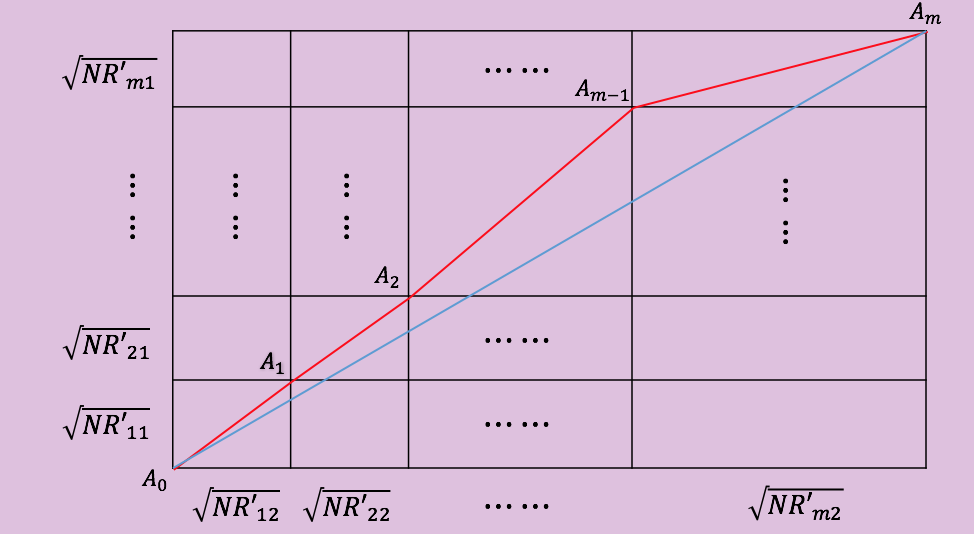
\includegraphics[width = 0.6\textwidth]{../common/m1.png}
   		 	\begin{tikzpicture}
\pgfmathsetmacro{\HEIGHT}{1.2}
\pgfmathsetmacro{\HDOT}{2.2}
\pgfmathsetmacro{\WDOT}{3.2}
\pgfmathsetmacro{\WOne}{1.6}
\pgfmathsetmacro{\WTwo}{2.2}
\pgfmathsetmacro{\WN}{4.2}

\pgfmathsetmacro{\LEN}{\WOne + \WTwo + \WN + \WDOT}
\pgfmathsetmacro{\TH}{3*\HEIGHT+ \HDOT}

\tikzset{
  t/.style={draw, on grid, align=center, minimum height=1ex},
  coord/.style={coordinate, on grid, node distance=6mm and 25mm},
  between/.style args={#1 and #2}{
         at = ($(#1)!0.5!(#2)$)
    }
}

\draw [name path=h1] (0, 0) -- (\LEN, 0);
\draw [name path=h2] (0, \HEIGHT) -- (\LEN, \HEIGHT);
\draw [name path=h3] (0, 2*\HEIGHT) -- (\LEN, 2*\HEIGHT);
\draw [name path=h4] (0, 2*\HEIGHT + \HDOT) -- (\LEN, 2*\HEIGHT + \HDOT);
\draw [name path=h5] (0, 3*\HEIGHT + \HDOT) -- (\LEN, 3*\HEIGHT + \HDOT);

\draw[name path=v1] (0, 0) -- (0, \TH);
\draw[name path=v2] (\WOne, 0) -- (\WOne, \TH);
\draw[name path=v3] (\WOne + \WTwo, 0) -- (\WOne + \WTwo, \TH);
\draw[name path=v4] (\WOne + \WTwo + \WDOT, 0) -- (\WOne + \WTwo + \WDOT, \TH);
\draw[name path=v5] (\WOne + \WTwo + \WDOT + \WN, 0) -- (\WOne + \WTwo + \WDOT + \WN, \TH);

\path [name intersections={of=h1 and v1,by=A0}];
\path [name intersections={of=h2 and v2,by=A1}];
\path [name intersections={of=h3 and v3,by=A2}];
\path [name intersections={of=h4 and v4,by=Am1}];
\path [name intersections={of=h5 and v5,by=Am}];

\draw [red] (A0) -- (A1) -- (A2) -- (Am1) -- (Am);
\draw [blue] (A0) -- (Am);

\node [below=0.01 of A0, anchor=north east] {$A_0$};
\node [above=0.05 of A1, anchor=south east]{$A_1$};
\node [above=0.05 of A2, anchor=south east] {$A_2$};
\node [above=0.05 of Am1, anchor=south east] {$A_{m-1}$};
\node [above=0.05 of Am, anchor=south]{$A_m$};


\path [name intersections={of=h1 and v1,by=t00}];
\path [name intersections={of=h2 and v1,by=t01}];
\path [name intersections={of=h3 and v1,by=t02}];
\path [name intersections={of=h4 and v1,by=t03}];
\path [name intersections={of=h5 and v1,by=t04}];
\node [coord, between=t00 and t01] (x1){};
\node [coord, between=t01 and t02] (x2){};
\node [coord, between=t02 and t03] (x3){};
\node [coord, between=t03 and t04] (x4){};

\node [left=0.05 of x1.west] {$\sqrt{{\nr}'_{11}}$};
\node [left=0.05 of x2.west] {$\sqrt{{\nr}'_{21}}$};
\node [left=0.7 of x3.west, anchor=center] {$\vdots$};
\node [left=0.05 of x4.west] {$\sqrt{{\nr}'_{m1}}$};

\path [name intersections={of=h1 and v1,by=s00}];
\path [name intersections={of=h1 and v2,by=s01}];
\path [name intersections={of=h1 and v3,by=s02}];
\path [name intersections={of=h1 and v4,by=s03}];
\path [name intersections={of=h1 and v5,by=s04}];
\node [coord, between=s00 and s01] (y1){};
\node [coord, between=s01 and s02] (y2){};
\node [coord, between=s02 and s03] (y3){};
\node [coord, between=s03 and s04] (y4){};

\node [below=0.5 of y1.south, anchor=center] {$\sqrt{{\nr}'_{12}}$};
\node [below=0.5 of y2.south, anchor=center] {$\sqrt{{\nr}'_{22}}$};
\node [below=0.5 of y3.south, anchor=center] {$\dots$};
\node [below=0.5 of y4.south, anchor=center] {$\sqrt{{\nr}'_{m2}}$};

\node at (x1.east -| y3.north) {$\dots$};
\node at (x2.east -| y3.north) {$\dots$};
\node at (x4.east -| y3.north) {$\dots$};

\node at (y1.north |- x3.east) {$\vdots$};
\node at (y2.north |- x3.east) {$\vdots$};
\node at (y4.north |- x3.east) {$\vdots$};

\end{tikzpicture}

   		 	\caption{Proof by shortest distance\label{fig:path}}
   		 \end{figure}
   As shown in Figure~\ref{fig:path}, we construct a grid whose length and width are divided into $m$ segments,  the $i$-th segment of which has length $\sqrt{\nr'_{i1}}$ and $\sqrt{\nr'_{i2}}$ respectively.

   	Then, $S_1^{'2}+S_2^{'2}=A_0A_m^2$, that is, equals to the square of the blue segment's length. In the meanwhile,
   	 $$S_1^2 = (\sum_{i=1}^m \sqrt{\nr_{i1}})^2 > (\sum_{i=1}^m \sqrt{\nr'_{i1}+\nr'_{i2}})^2 = (\sum_{i=1}^m A_{i-1}A_i)^2$$,
   	 which equals to the sum of squares of all red segments. Since the shortest distance between two points is a line-segment, it holds that $S_1^2 >S_1^{'2}+S_2^{'2}$.

   	 For the cases where $k>2$ DApps are split, 	we can regard it as successive splits and iteratively use the result on $k=2$.

   	 So the property is proved.

\end{proof}

\subsection{Proof of Corollary~\ref{c1}}
\label{subsection:proof3}
\begin{proof}
	For any voter that is bought over by $d_1$'s developer, before splitting, we
	can regard the voter as a normal voter who values all DApps with weight
	vector $(1,0,0,\ldots,0)$, as he gives his all voting capacity to $d_1$.
	Suppose now $d_1$ is split into $k$ DApps and the bough-over voter's
	contributory values to the $k$ DApps are $\nr_{t1},\ldots,\nr_{tk}$, whose
	sum is fixed. According to the condition that the equality holds for Cauthy's
	inequality in the proof of Property~\ref{p1}, the voter can be regard as a
	normal voter who values all DApps with weight vector
	$(\sqrt{\nr_{t1}}/C,\sqrt{\nr_{t2}}/C,\ldots, \sqrt{\nr_{tk}}/C,0,0,\ldots,0)$, where $C=\sum_{j=1}^k \sqrt{\nr_{tj}}$. That is, the voter values the split DApps with weights according to kind of proportion and values all other DApps with 0 weights.~\footnote{Note that scaling all weights by a constant does not effect the results, since the total contributory value of the voter only depends on the proportions of weights to total weights}. Since
		$$\sum_{j=1}^k \sqrt{\nr_{tj}}/C =1$$
	so the case in this corollary can be reduced to the case about normal voters(Property~\ref{p2}). So the corollary is proved.
\end{proof}

\subsection{Proof of Property~\ref{p3}}
\begin{proof}
	We first consider the case that a voter splits his account into two sub-accounts. We fix the actions of other voters. Let $c$ to be the original account and $a,b$ to be the split sun-accounts, $S,S'$ to be the ranking score of the DApp that the voter plans to vote before and after splitting respectively, $U,U'$ to be the final reward of the developer of the DApp that the voter plans to vote before and after splitting respectively. By definition, we have
	$$S= \sqrt{\nr_c}+O,\quad S'=\sqrt{\nr_a}+\sqrt{\nr_b}+O$$,
	where $O$ is the sum of contributory values by other voters, which is fixed.

	By ~\ref{eq:sqrt_nr} it holds that $S < S'$. That is, the rank of the DApp does not increase.

	In the meanwhile, by definition,
	$$U = \frac{S}{S+P}\lambda M,\quad U' = \frac{S'}{S'+P} \lambda M$$,
	where $P$ is the sum of squares of other DApp's ranking score, which is fixed.

	Since $S < S'$ it holds that $U \leq U'$. That is the developer's final reward does not increase.

	For the cases where $k>2$ sub-accounts are split, we can regard it as successive splits and iteratively use the result on $k=2$.

\end{proof}
